\documentclass{beamer}
%
% Choose how your presentation looks.
%
% For more themes, color themes and font themes, see:
% http://deic.uab.es/~iblanes/beamer_gallery/index_by_theme.html
%
\mode<presentation>
{
  \usetheme{default}      % or try Darmstadt, Madrid, Warsaw, ...
  \usecolortheme{default} % or try albatross, beaver, crane, ...
  \usefonttheme{default}  % or try serif, structurebold, ...
  \setbeamertemplate{navigation symbols}{}
  \setbeamertemplate{caption}[numbered]
} 

\usepackage[english]{babel}
\usepackage[utf8x]{inputenc}

\title[Your Short Title]{Flood risk prediction via machine learning methods}
\author{Vladislav Pyzh}
\institute{MIPT}
\date{}

\begin{document}

\begin{frame}
  \titlepage
\end{frame}

% Uncomment these lines for an automatically generated outline.
%\begin{frame}{Outline}
%  \tableofcontents
%\end{frame}

\section{Some \LaTeX{} Examples}

\subsection{Data and short results}

\begin{frame}{Data and short results}

% Commands to include a figure:

% \begin{figure}
% \centering
% \begin{minipage}{.7\textwidth}
%   \centering
%   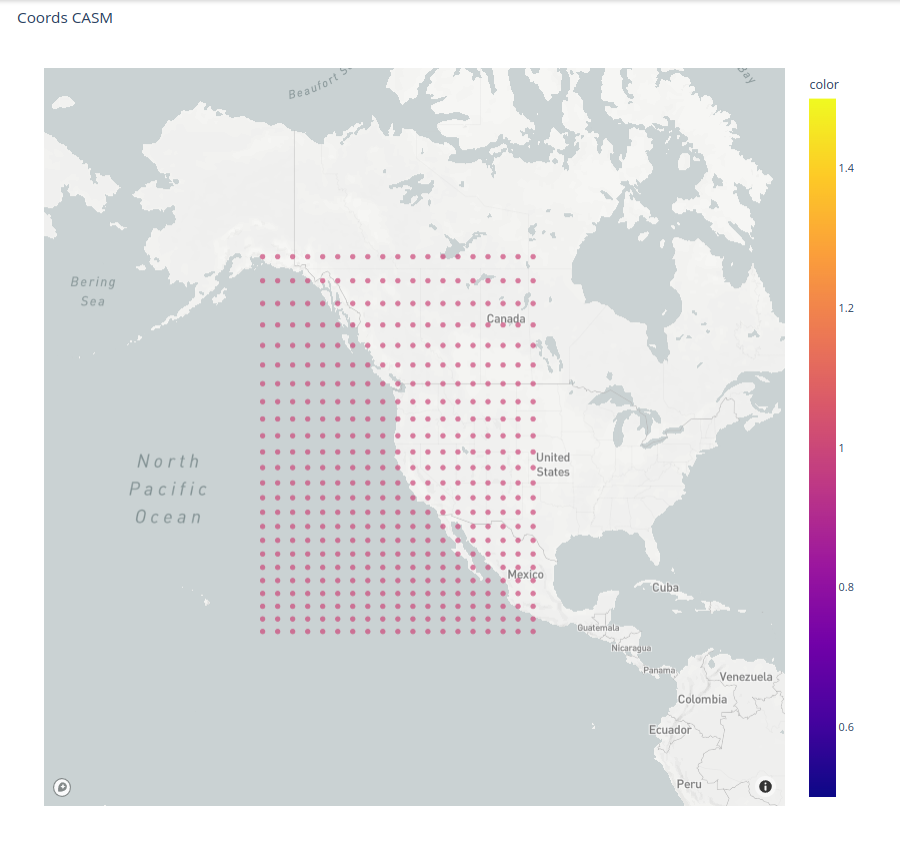
\includegraphics[width=.7\linewidth]{map.png}
%   \\\captionof{figure}
%   \label{fig:test1}
% \end{minipage}%
% \begin{minipage}{.7\textwidth}
%   \centering
%   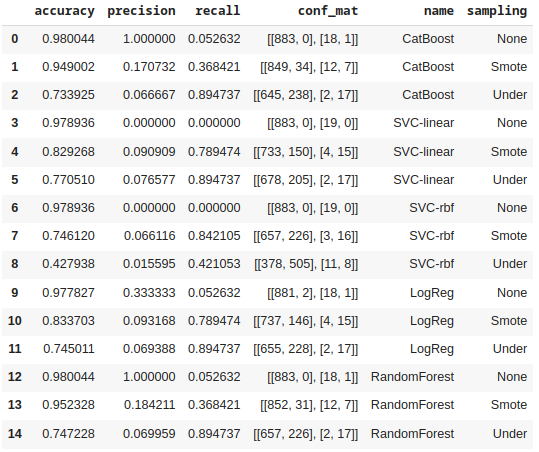
\includegraphics[width=.7\linewidth]{pivot_table.png}
%   \\\captionof{figure}
%   \label{fig:test2}
% \end{minipage}
% \end{figure}

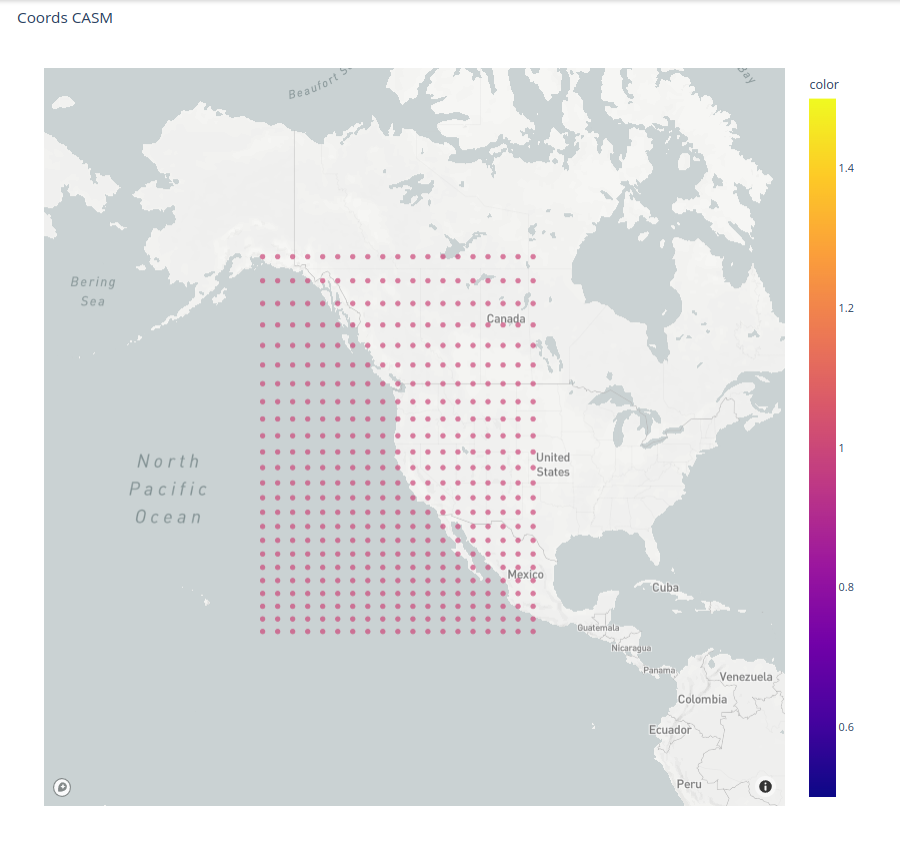
\includegraphics[width=0.45\textwidth]{map.png}
\hfill
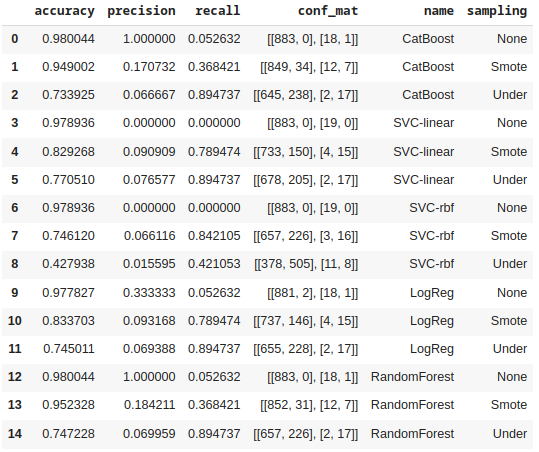
\includegraphics[width=0.45\textwidth]{pivot_table.png}

\end{frame}

\end{document}
